\documentclass[dvipsnames]{article}

\usepackage{amsfonts}
\usepackage{amsmath}
\usepackage{amsthm}
\usepackage{cases}
\usepackage{float}
\usepackage{graphicx}
\usepackage{listings}
\usepackage{pgfplots}
\usepackage{pxfonts}
\usepackage{subcaption}
\usepackage{subfiles}
\usepackage{xcolor}

\theoremstyle{definition}
\newtheorem{definition}{Definizione}

\definecolor{backcolour}{rgb}{0.95,0.95,0.92}

\lstdefinelanguage{ps}{
    morekeywords=[1]{function, true},
    morekeywords=[2]{set, while, for, return, if, else},
    morekeywords=[3]{assert, swap, max, min, random, randomInt, randomFrom, push, pop},
    morecomment=[l]{//},
    sensitive=true
}
\lstset{
    backgroundcolor=\color{backcolour},
    keywordstyle=[1]\color{Blue},
    keywordstyle=[2]\color{DarkOrchid},
    keywordstyle=[3]\color{Blue},
    numberstyle=\scriptsize\color{darkgray},
    commentstyle=\color{ForestGreen},
    basicstyle=\ttfamily\small,
    numbers=left,
    numbersep=5pt,
    language=ps
}

\pgfplotsset{compat=1.18}
\pgfplotsset{colormap={rs}{color(0)=(white) color(1)=(red!50!lightgray) color=(red)}}

\newcommand{\makeaxis}[2]{
    \begin{minipage}{0.4\paperwidth}
        \begin{tikzpicture}
            \begin{axis} [
                title={#1}
            ]
                \addplot+ [
                    scatter,
                    only marks,
                    scatter src={\thisrow{freq}/\thisrow{max_freq}}
                    ] table [x=n,y=value] {#2};
            \end{axis}
        \end{tikzpicture}
    \end{minipage}
}

\newcommand{\makefigure}[2]{
    \begin{figure}[H]
        \makebox[\textwidth]{
            \expandafter\makeaxis{Generatore esaustivo}{data/exh_gen_#2.dat}
            \hfill
            \expandafter\makeaxis{Generatore esaustivo con flitro}{data/exh_filt_gen_#2.dat}
        }
        \vskip\baselineskip
        \makebox[\textwidth]{
            \expandafter\makeaxis{Generatore casuale con filtro}{data/rand_filt_gen_#2.dat}
            \hfill
            \expandafter\makeaxis{Generatore a intervalli}{data/int_filt_gen_#2.dat}
        }
        \makebox[\textwidth]{
            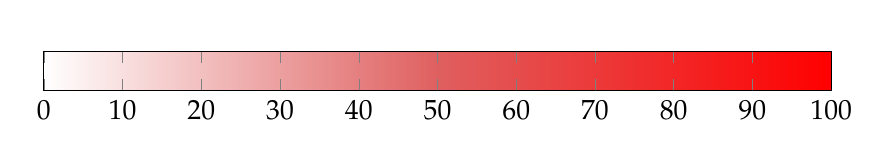
\begin{tikzpicture}
                \begin{axis}[
                    hide axis,
                    scale only axis,
                    height=0pt,
                    width=0pt,
                    colormap name=rs,
                    colorbar horizontal,
                    point meta min=0,
                    point meta max=100,
                    colorbar style={
                        width=10cm,
                        xtick={0,10,...,100}
                    }
                ]
                    \addplot [draw=none] coordinates {(0,0)};
                \end{axis}
            \end{tikzpicture}
        }
        \caption{#1}
    \end{figure}
}